\documentclass[11pt,onside,a4paper,fleqn]{report}            
\usepackage{graphicx}
\usepackage{epstopdf}
\usepackage{placeins}
\usepackage{amsmath}
\usepackage{array}
\usepackage{booktabs}
\makeatletter
\renewcommand\arraystretch{2.5}
\renewcommand\normalsize{%
\@setfontsize\normalsize\@xpt\@xiipt
   \abovedisplayskip 4\p@ \@plus2\p@ \@minus8\p@
   \abovedisplayshortskip \z@ \@plus6\p@
   \belowdisplayshortskip 4\p@ \@plus3\p@ \@minus3\p@
   \belowdisplayskip \abovedisplayskip
   \let\@listi\@listI}
\makeatother
 
 
\parindent0pt  \parskip10pt             % make block paragraphs
                           				% do not right-justify
\title{\bf Golang Tendency Analysis Report}  % Supply information
\author{ \\ \\*mayuke\\}
              							%   for the title page.
\date{\today}                           %   Use current date.
 
\begin{document}                        % End of preamble, start of text.
\maketitle                              % Print title page.
\begin{abstract}

%Abstract
Golang was publicly announced in November 2009 and version 1.0 was released in March 2012. Now Go is widely used in production at Google and in many other organizations and open-source projects.In order to study the development trend of Go language in recent years, this report uses the API provided by Github to obtain a certain amount of repositories information from Github and show the development and changes of Go language from its birth to the present from several different perspectives.

\end{abstract}
\pagenumbering{roman}                   % roman page number for toc
\setcounter{page}{1}                    % make it start with "1"
\pagenumbering{arabic}					% Start text with arabic 1
\chapter{Introduction}
This report shows the development trend of Go from three different perspectives:
\begin{itemize}
\item Nearly 1,000 Github repositories are randomly selected each year from 2009 to 2021, and the number of repositories where language is Go is analyzed to reflect the change of popluarity of Go language.

\item The repositories built by Go language during the five years from 2017 to 2021 are selected, and the commit information of each repositories is obtained and made into a calendar 
heat map to reflect the changes in Go language user activity.

\item Crawl all description information of the repositories obtained during the five years from 2017 to 2021 and make into wordcloud map after word segmentation, so as to analyze
 the change of keywords of Go language in different years.
\end{itemize}

%\section{Objective}
 
\chapter{Implemention}

\section{The number of repositories changes over time}
\paragraph{} The change of the popularity of Go language over time can be reflected from one aspect by studying the change of the number of repositories using Go language over time. Based on this, the project uses Simple random sampling method to randomly select a certain number of repositories from Github every year and count the number of Go language repositories.

\subsection{raw data}
\paragraph{} The project uses the Github API to acquire approximately 1,200 repositories per year from 2009 to 2021, for a total of approximately 15,000 repositories, and counts Go and three other programming languages that are currently popular
C++, Python, Java repositories number.

\paragraph{} The data results are as follows:

% Data Table
\begin{table}[ht]
\renewcommand{\arraystretch}{1.3}
\begin{tabular}{@{}llllllllllllll@{}}
\toprule
years  & 09 & 10 & 11 & 12 & 13 & 14 & 15 & 16 & 17 & 18 & 19 & 20 & 21 \\ \midrule
Go     & 5    & 7    & 14   & 19   & 37   & 55   & 58   & 54   & 59   & 70   & 61   & 57   & 69   \\
C++    & 32   & 45   & 68   & 65   & 75   & 61   & 65   & 66   & 52   & 68   & 53   & 71   & 48   \\
Java   & 43   & 67   & 87   & 86   & 97   & 121  & 143  & 129  & 95   & 68   & 59   & 45   & 35   \\
Python & 139  & 166  & 155  & 141  & 124  & 120  & 117  & 151  & 208  & 243  & 255  & 253  & 249  \\ \bottomrule
\end{tabular}
\caption{The number of repositories in different languages per 1000 repositories}
\end{table}

\paragraph{} This data is plotted into line chart 2.1, which visually shows how the four programming languages changed between 2009 and 2021.It can be simply shown in the figure that the number of Go language repositories has been on the rise, which indicates that Go
Languages are becoming more and more popular in recent years.

%figure 2.1
\begin{figure}[ht]
\centering
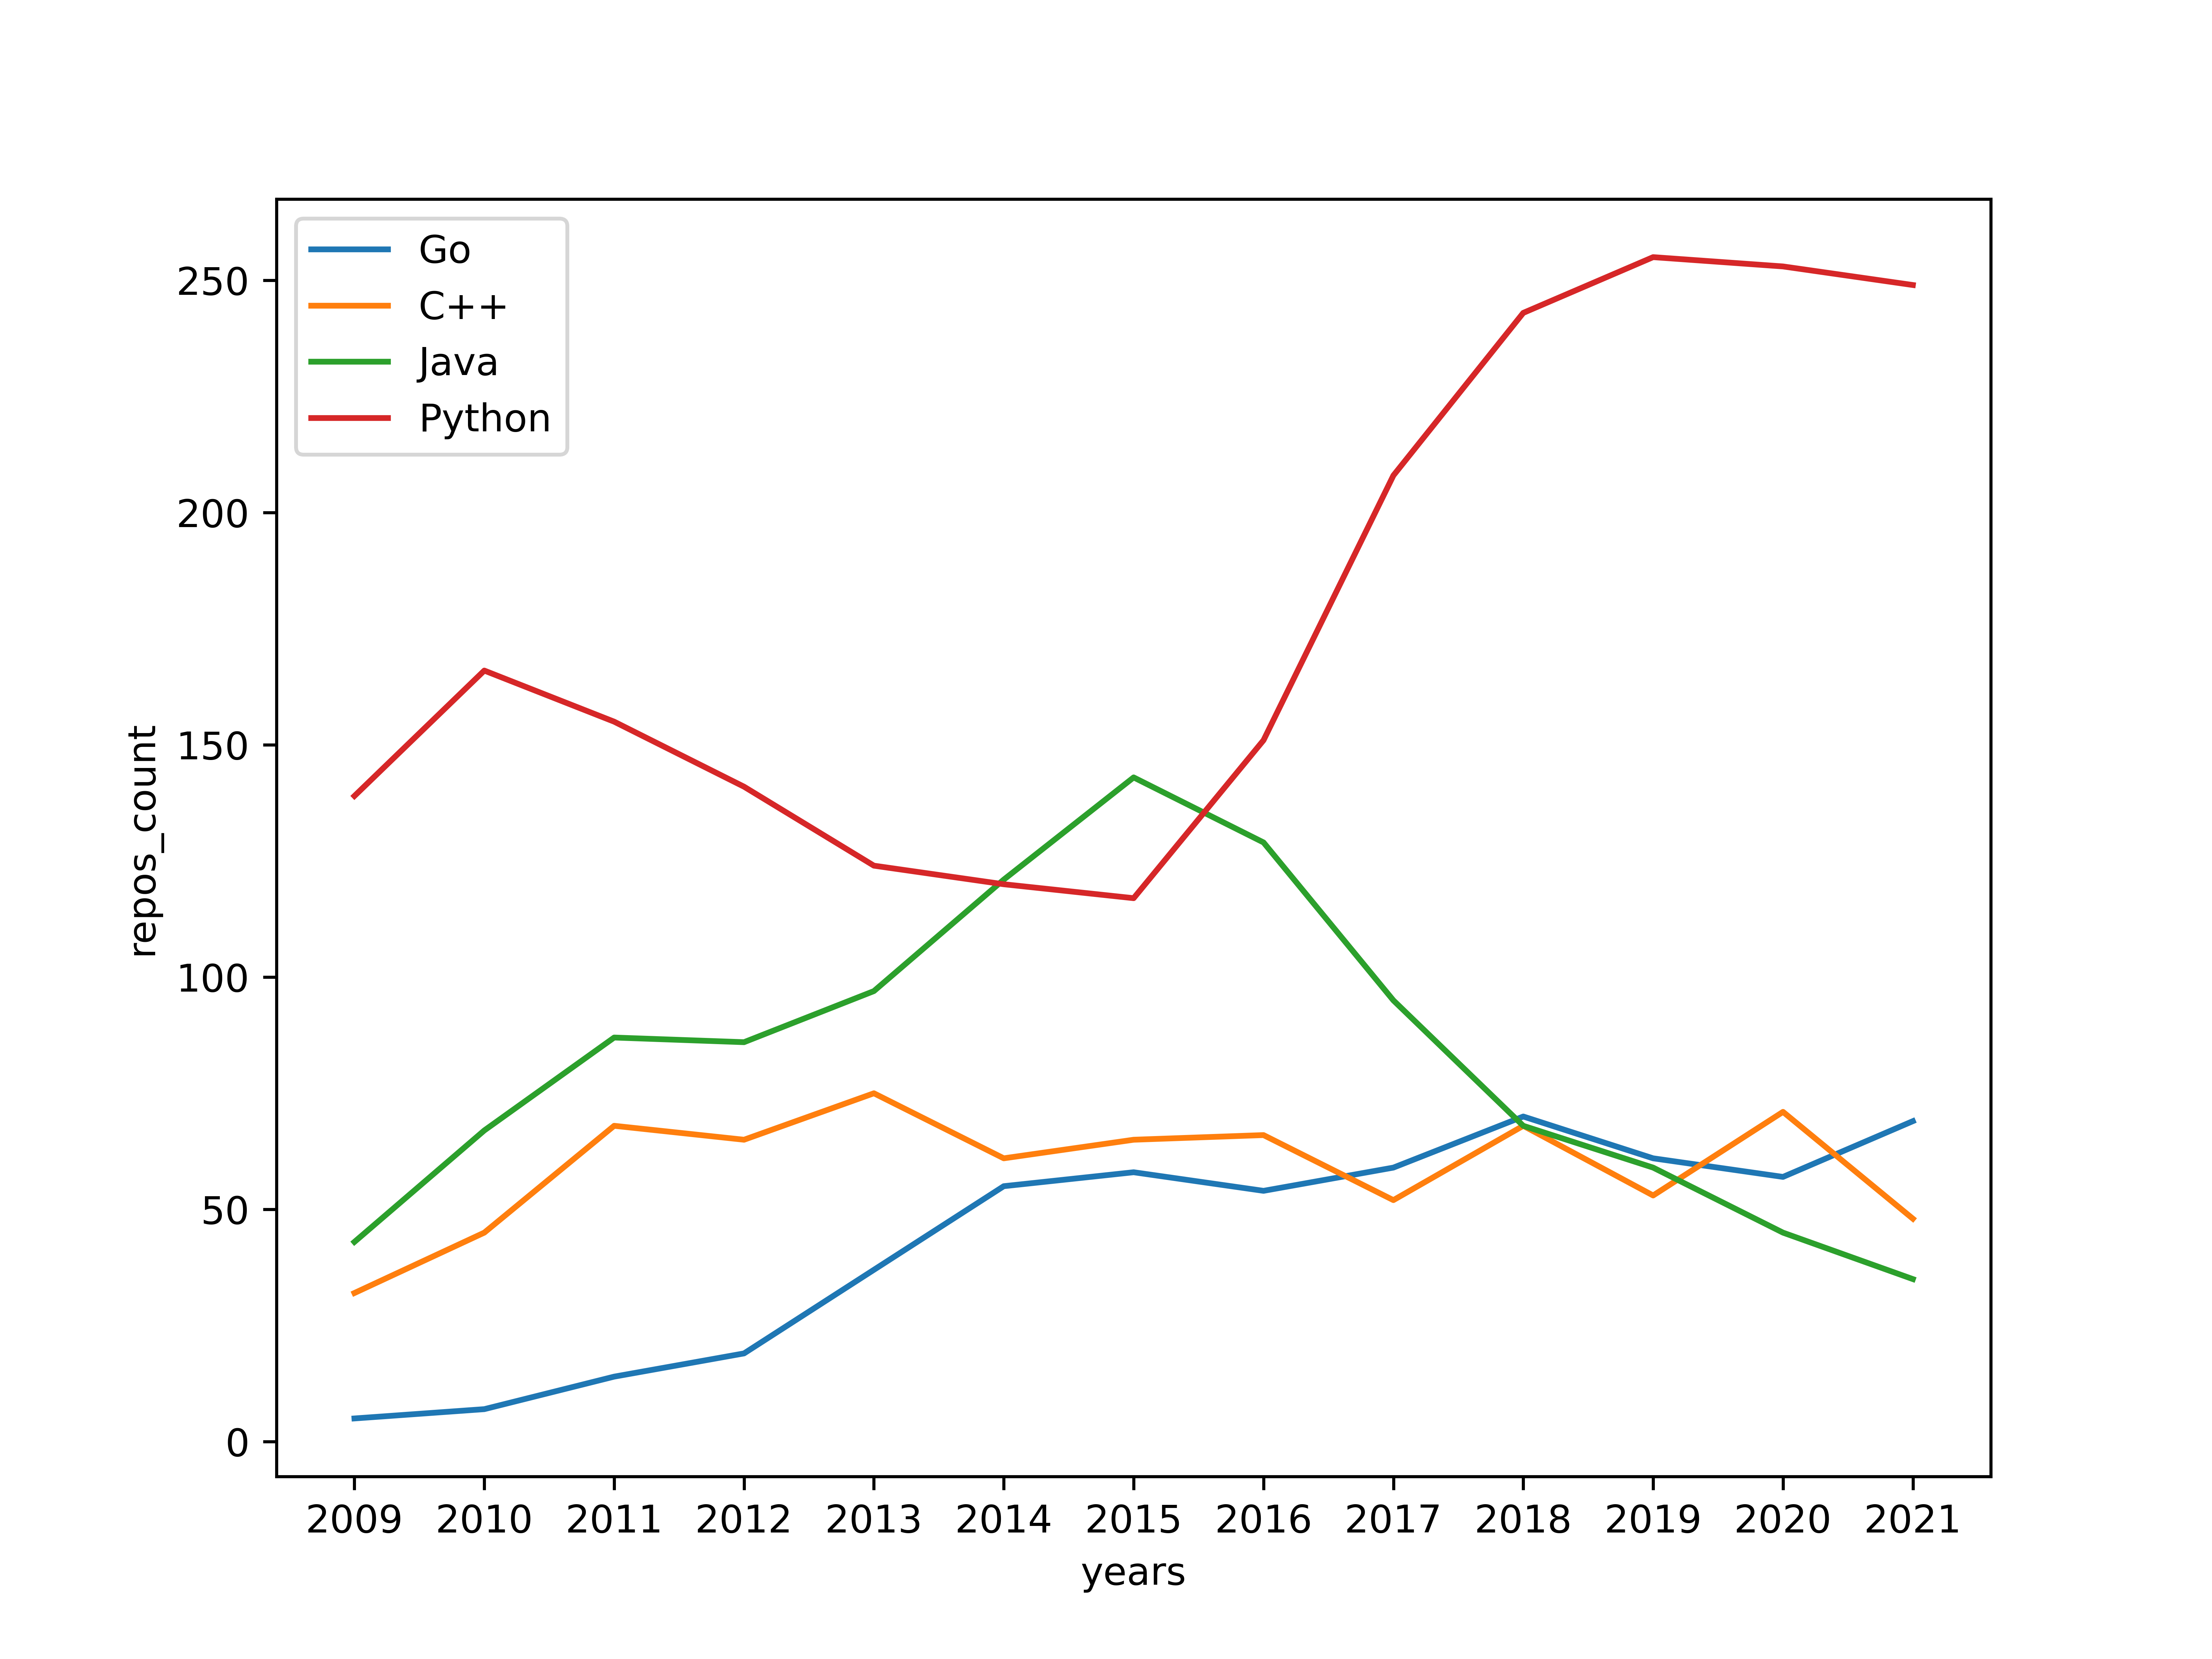
\includegraphics[scale=0.6]{result/yearsChange.png}
\caption{The number of repositories varies by programming language}
\label{fig:pathdemo4}
\end{figure}

\subsection{Programming language popularity}

%figure 2.2
\begin{figure}[ht]
\centering
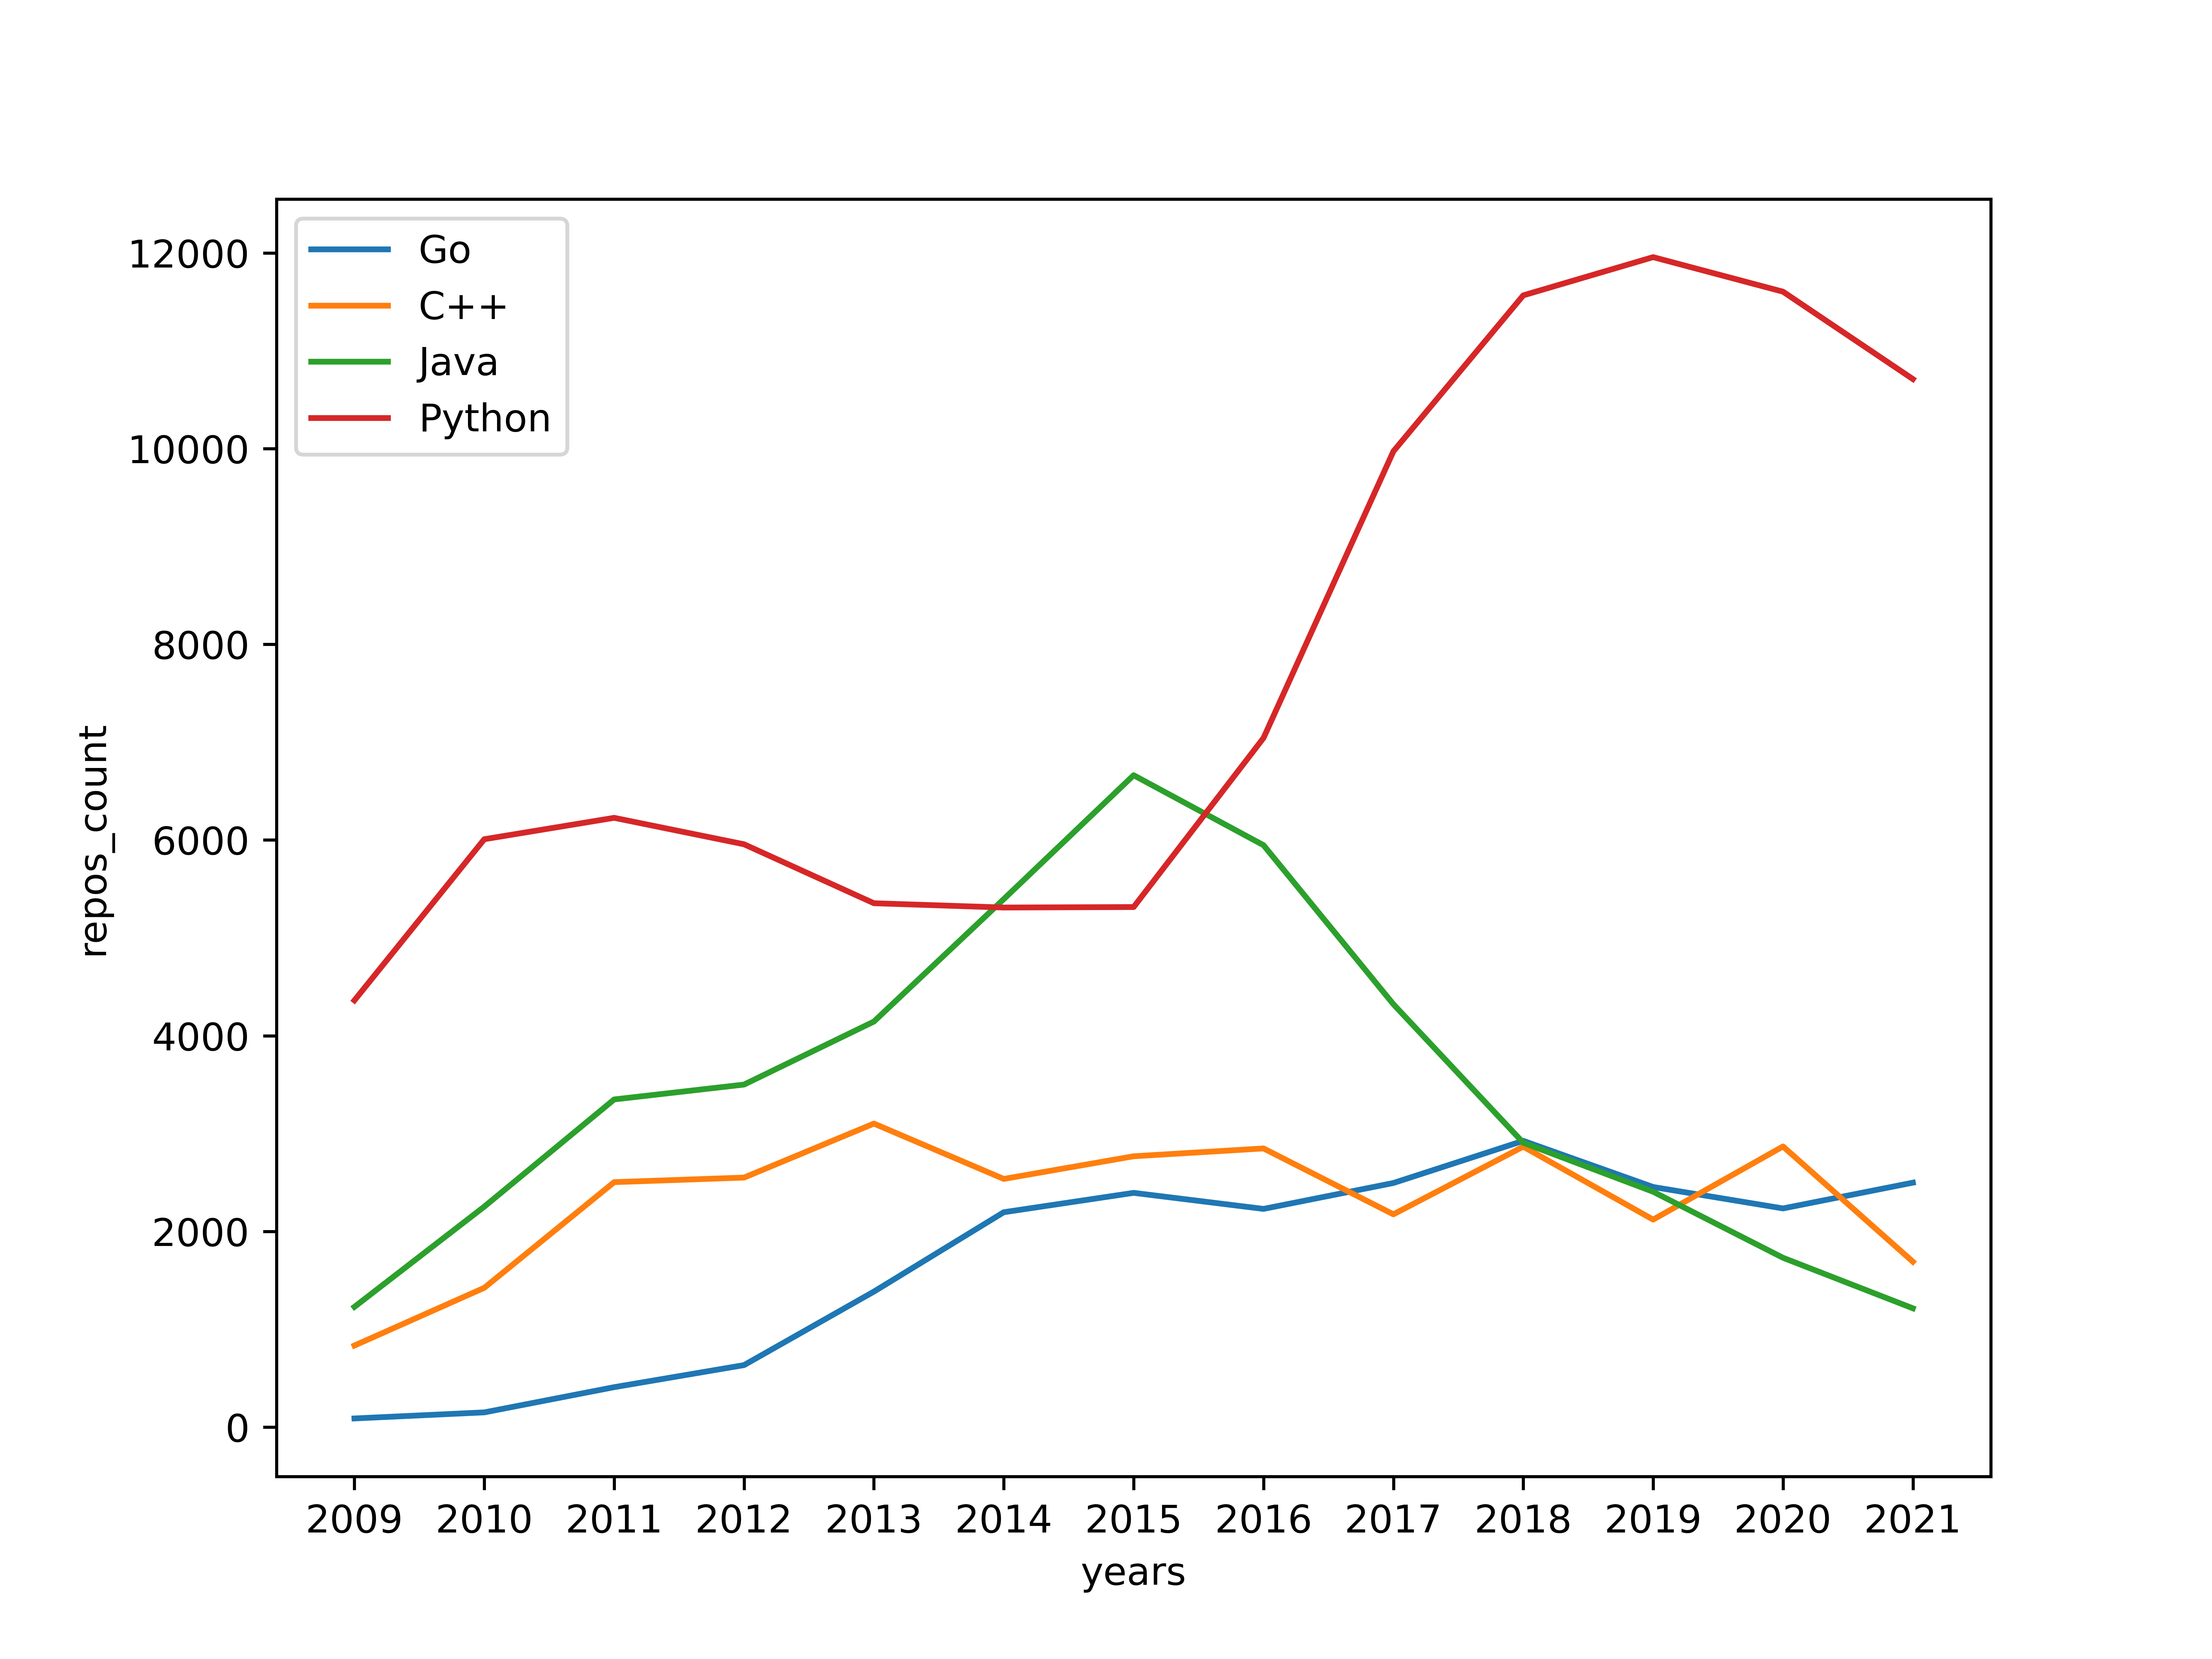
\includegraphics[scale=0.6]{result/yearsChange_modifed.png}
\caption{Programming language popularity changes over time}
\label{fig:pathdemo4}
\end{figure}




\section{analysis2}
 
\section{analysis3}
 
 
 
\chapter{Analysis}
\hspace{0.8cm}
\section{Conclution}                  % Print a "section" heading
\hspace{0.8cm}
\end{document}                          % The required last line